\section{Aktør-kontekst}
Applikationen har 4 forskellige aktører, 3 primære og 1 sekundær, som kan ses herunder på figur \ref{fig:aktor_konteks}.
\begin{figure}[H]
  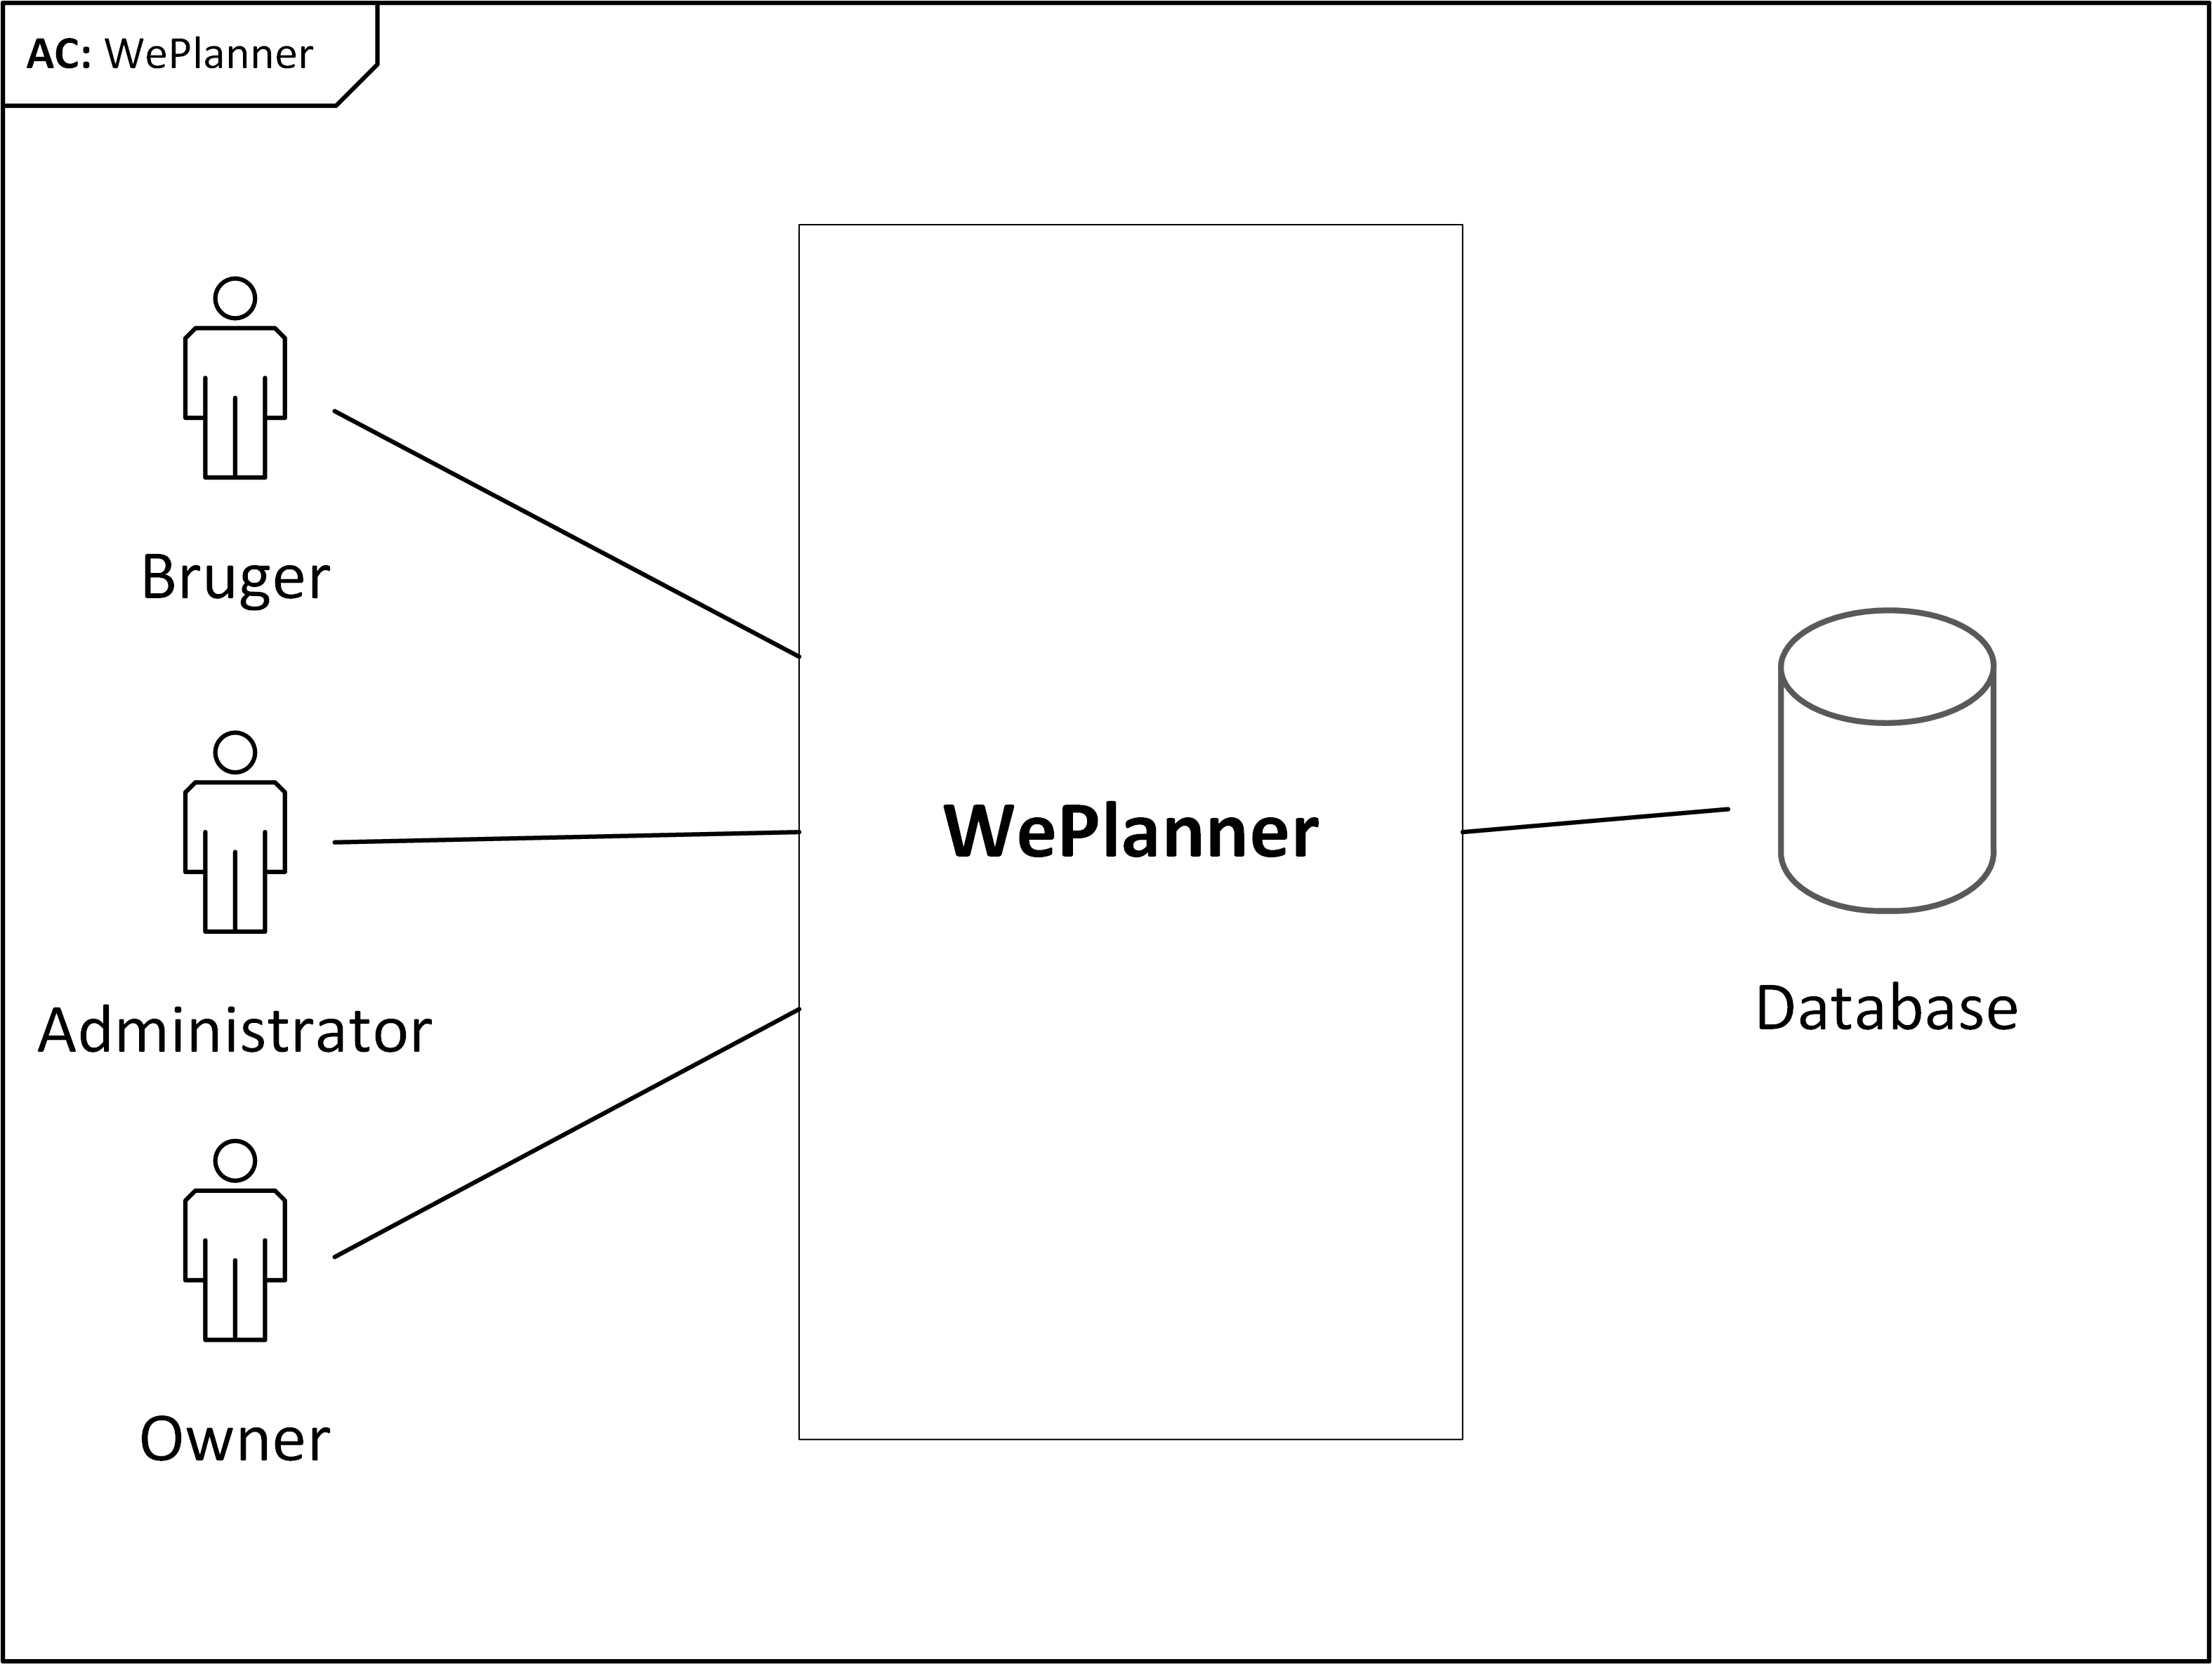
\includegraphics[width=\linewidth]{01_Billeder/05_Kravspek/Aktor-kontekst_diagram.png}
  \caption{Aktør-kontekst diagram for WePlanner}
  \label{fig:aktor_konteks}
\end{figure}
Alle aktørernes rettigheder kan ses på tabel \ref{tab:rettighedtabel}.
\subsection{Bruger:}
Aktøren "bruger", er en person som har oprettet et brugerlogin til WePlanner, og dermed kan logge sig ind på siden.

\subsection{Owner:}
"Owner" er brugeren som har oprettet gruppen, og en gruppe vil derfor altid kun have én owner. Owneren kan de samme ting som en bruger, men har ophøjede rettigheder. 

\subsection{Administrator:}
En administrator har på samme måde som owner, ophøjede rettigheder, og kan moderere indhold for en gruppe. 

\subsection{Database:}
Databasen er SQL-baseret, og indeholder informationerne for alle brugere og grupper. Det er her der bliver gemt loginoplysninger for brugere, og også her alle widgets for de individuelle grupper vil blive gemt.

\subsection{Rettighedstabel}
For at klargøre rettighederne for bruger, administrator og owner er disse opstillet i tabel \ref{tab:rettighedtabel}.

\begin{table}[h]
\centering
\begin{tabular}{lccc}
\cline{2-4}
\multicolumn{1}{l|}{}                                                                                                         & \multicolumn{1}{l|}{\textbf{Bruger}} & \multicolumn{1}{l|}{\textbf{Administrator}} & \multicolumn{1}{l|}{\textbf{Owner}} \\ \hline
\multicolumn{1}{|l|}{\textbf{Tilføje Widget}}                                                                                 & \multicolumn{1}{c|}{X}               & \multicolumn{1}{c|}{X}                      & \multicolumn{1}{c|}{X}              \\ \hline
\multicolumn{1}{|l|}{\textbf{Fjern Widget}}                                                                                   & \multicolumn{1}{c|}{}                & \multicolumn{1}{c|}{X}                      & \multicolumn{1}{c|}{X}              \\ \hline
\multicolumn{1}{|l|}{\textbf{Redigér indhold i Widget}}                                                                                 & \multicolumn{1}{c|}{X}               & \multicolumn{1}{c|}{X}                      & \multicolumn{1}{c|}{X}              \\ \hline
\multicolumn{1}{|l|}{\textbf{Log ind}}                                                                                        & \multicolumn{1}{c|}{X}               & \multicolumn{1}{c|}{X}                      & \multicolumn{1}{c|}{X}              \\ \hline
\multicolumn{1}{|l|}{\textbf{Indstil brugerindstillinger}}                                                                    & \multicolumn{1}{c|}{X}               & \multicolumn{1}{c|}{X}                      & \multicolumn{1}{c|}{X}              \\ \hline
\multicolumn{1}{|l|}{\textbf{\begin{tabular}[c]{@{}l@{}}Indstille gruppeindstillinger\\ (Gruppenavn mm.)\end{tabular}}} & \multicolumn{1}{c|}{}                & \multicolumn{1}{c|}{X}                      & \multicolumn{1}{c|}{X}              \\ \hline
\multicolumn{1}{|l|}{\textbf{Fjern bruger fra gruppe}}                                                                                   & \multicolumn{1}{c|}{}                & \multicolumn{1}{c|}{X}                      & \multicolumn{1}{c|}{X}              \\ \hline
\multicolumn{1}{|l|}{\textbf{Tilføje Administrator}}                                                                          & \multicolumn{1}{c|}{}                & \multicolumn{1}{c|}{X}                       & \multicolumn{1}{c|}{X}              \\ \hline
\multicolumn{1}{|l|}{\textbf{Fjerne Administrator}}                                                                           & \multicolumn{1}{c|}{}                & \multicolumn{1}{c|}{X}                       & \multicolumn{1}{c|}{X}              \\ \hline
\multicolumn{1}{|l|}{\textbf{Videregive Owner rolle}}                                                                           & \multicolumn{1}{c|}{}                & \multicolumn{1}{c|}{}                       & \multicolumn{1}{c|}{X}              \\ \hline
\multicolumn{1}{|l|}{\textbf{Slette gruppe}}                                                                           & \multicolumn{1}{c|}{}                & \multicolumn{1}{c|}{}                       & \multicolumn{1}{c|}{X}              \\ \hline
\end{tabular}
\caption{Tabel som viser hvad de forskellige aktører har adgang til i en gruppe. Brugere kan kun redigere i indhold som de selv har oprettet.}
    \label{tab:rettighedtabel}
\end{table}

